\section{Auswertung}
\label{sec:Auswertung}
\newcommand{\kleineKugelDurchmesser}{\SI{15.61}{\milli\meter} }
\newcommand{\kleineKugelRadius}{\SI{0.007805}{\meter} }
\newcommand{\kleineKugelMasse}{\SI{0.0044531}{\kilo\gram} }
\newcommand{\kleineKugelDichte}{\SI{2235.91}{\kilo\gram\per\cubic\meter} }

\newcommand{\grosseKugelRadius}{\SI{0.00789}{\meter} }
\newcommand{\grosseKugelDurchmesser}{\SI{0.01578}{\meter} }
\newcommand{\grosseKugelMasse}{\SI{0.0049528}{\kilo\gram} }
\newcommand{\grosseKugelDichte}{\SI{2407.31}{\kilo\gram\per\cubic\meter} }

Bei der kleinen Kugel wurde ein Durchmesser von \kleineKugelDurchmesser beziehungsweise ein Radius von \kleineKugelRadius gemessen.
Daraus lässt sich zusammen mit einer Masse von \kleineKugelMasse eine Dichte von
\begin{equation*}
  \rho_\text{k}
  = \frac{m_\text{k}}{V_\text{k}}
  = \frac{m_\text{k}}{\frac{4}{3}\pi r_\text{k}^3}
  = \frac{\kleineKugelMasse}{\frac{4}{3}\pi\times(\kleineKugelRadius)^3}
  = \kleineKugelDichte
\end{equation*}
berechnen.
Äquivalent lässt sich für die große Kugel mit einem Radius von \grosseKugelRadius und einer Masse von \grosseKugelMasse die Dichte berechnen.
\begin{equation*}
  \rho_\text{k}
  = \frac{m_\text{g}}{V_\text{g}}
  = \frac{m_\text{g}}{\frac{4}{3}\pi r_\text{g}^3}
  = \frac{\grosseKugelMasse}{\frac{4}{3}\pi\times(\grosseKugelRadius)^3}
  = \grosseKugelDichte.
\end{equation*}

\begin{table}
  \centering
  \input{build/kleine_kugel.tex}
  \caption{Messwerte der Fallzeit der kleinen Kugel bei Raumtemperatur.}
  \label{tab:kleine_kugel}
\end{table}

\noindent In Tabelle \autoref{tab:kleine_kugel} sind die Messwerte der Fallzeit der kleinen Kugel aufgeführt.
Diese werden gemittelt und die Standartabweichung wird gebildet.
\begin{equation*}
  t_{k} = \frac{1}{N} \sum_{i=1}^{N}x_i =  \SI{12.80}{\second}
\end{equation*}
\begin{equation*}
  \Delta t_{k} = \sqrt{\bar{x²}-\bar{x}²} = \SI{0.12}{\second}
\end{equation*}
Sodass mit der Zeit $t_{k}$ gerechnet werden kann.

\begin{table}
  \centering
  \input{build/grosse_kugel.tex}
  \caption{Messwerte der Fallzeit der großen Kugel bei Raumtemperatur.}
  \label{tab:grosse_kugel}
\end{table}

\noindent Mit der gegebenen Apparaturkonstante

\begin{equation*}
  K_\text{k} = \SI{0.07640e-6}{\pascal\cubic\meter\per\kilo\gram}
\end{equation*}
für die kleine Kugel und der Dichte von Wasser \cite{TfCuP}

\begin{equation*}
  \rho_\text{W} = \SI{998.2}{\kilo\gram\per\cubic\meter}
\end{equation*}
folgt bei Raumtemperatur $T=\SI{292,15}{\kelvin}$ über die Formel
\begin{equation*}
  \eta_\text{W} = (\rho_\text{k}-\rho_\text{W})K_\text{k} \cdot t_\text{k}
\end{equation*}
die Viskosität des destillierten Wassers

\begin{equation*}
  \eta_\text{W} = \SI{1.21(1)e-3}{\pascal\second}.
\end{equation*}


\subsection{Apparaturkonstante}

Die Messung der Temperaturabhängigkeit wird mit der großen Kugel durchgeführt,
weshalb zunächst die Apparaturkonstante für diese Kugel bestimmt werden muss. In Tabelle \ref{tab:grosse_kugel} sind die Messwerte der Fallzeit der großen
Kugel aufgeführt. Der Mittelwert der zehn Werte beträgt

\begin{equation*}
  t_\text{g} = \SI{48.45}{\second}
\end{equation*}
und die Standartabweichung beträgt
\begin{equation*}
  \Delta t_{k} = \sqrt{\bar{x²}-\bar{x}²} = \SI{0.70}{\second}.
\end{equation*}
Über die berechneten Dichten, die Fallzeit und die Viskosität $\eta_\text{W}$
von Wasser folgt bei Raumtemperatur die Apparaturkonstante

\begin{equation*}
  K_\text{g} = \frac{\eta_\text{W}}{t(\rho_\text{g}-\rho_\text{W})}
  = \SI{1.77e-8}{\pascal\cubic\meter\per\kilo\gram}
\end{equation*}
für die große Kugel.


\subsection{Temperaturabhängigkeit der Viskosität}

\begin{table}
  \centering
  \input{build/grosse_kugel_temperatur.tex}
  \caption{Messwerte der Fallzeit der großen Kugel bei verschiedenen Temperaturen.}
  \label{tab:grosse_kugel_temprature}
\end{table}

\noindent In \autoref{tab:grosse_kugel_temprature} sind die Messwerte der Fallzeiten für verschiedene Temperaturen angegeben.


\noindent Aus den Werten für die Fallzeit $t$ kann über die Formel \eqref{eq:viskositaet} die Viskosität für die jeweiligen Temperaturen bestimmt werden.
In Abbildung \ref{fig:grosse_kugel_temperatur} sind die experimentell bestimmten Werte für $\ln{\left( \frac{\eta}{\eta_0}\right)} $ gegen $1/T$ aufgetragen.
$\eta_0 = \SI{1}{mPa \, s}$ wird dabei genutzt, damit kein Logarithmus aus einer einheitenbehafteten Größe gebildet wird.

\noindent Die Ausgleichsgerade ist eine Funktion der Form
\begin{equation*}
  \ln{\left( \frac{\eta}{\eta_0}\right)} = \ln{\left( \frac{A}{\eta_0}\right)} + B \cdot \frac{1}{T} \quad, 
\end{equation*}
dessen Parameter zu 

\begin{align*}
  \ln{\left( \frac{A}{\eta_0}\right)} &= \num{-5.937 +- 0.129 } \\
  \implies \quad A &= \SI{2.64(34)e-3}{mPa \, s}
\end{align*}
und

\begin{equation*}
  B = \SI{1797.156 +- 39.780}{K}
\end{equation*}
bestimmt wurden.
Damit lautet die Funktion der Viskosität von der Temperatur
\begin{equation*}
  \eta(T) = (\num{2.64(34)e-3}) \exp\left(\frac{\SI{1797.156 +- 39.780}{K}}{T}\right) \si{\milli\pascal\second}.
\end{equation*}

\begin{figure}[H]
  \centering
  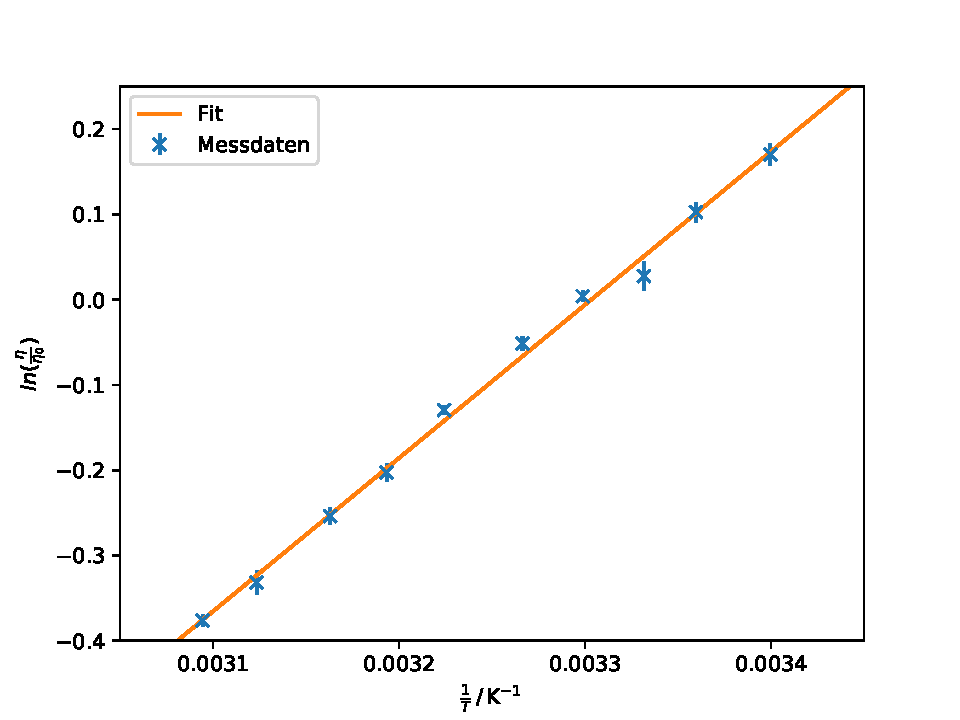
\includegraphics[]{assets/plot_1.pdf}
  \caption{Viskosität $\eta$ in Abhängigkeit von $t$}
  \label{fig:grosse_kugel_temperatur}
\end{figure}




\subsection{Reynolds-Zahl}

Die Reynolds-Zahl des destillierten Wassers kann mit Hilfe der gemessenen Viskosität, der Dichte des Wassers \cite{TfCuP},
der Fallrohrdicke, die etwa dem Durchmesser der großen Kugel
\begin{equation*}
  d_\text{g} = 2 r_\text{g} = \grosseKugelDurchmesser
\end{equation*}
entspricht, und der Geschwindigkeit der großen Kugel
\begin{equation*}
  v = \frac{l}{t}
\end{equation*}
bestimmt werden.

\begin{table}
  \centering
  \input{build/reynolds.tex}
  \caption{Die Reynold Zahlen der grossen Kugel in Abhängigkeit von der Temperatur.}
  \label{tab:grosse_kugel_reynold}
\end{table}